\documentclass[12pts]{report}

\usepackage[margin=1in]{geometry}
\usepackage[usenames, dvipsnames]{color}
\usepackage{setspace}
\usepackage{graphicx}
\doublespacing
\usepackage{fancyvrb}
\usepackage{varwidth}
\usepackage{verbatim}
\usepackage{multicol}
\usepackage{hyperref}

\setlength{\parindent}{0pt}
\setlength{\columnseprule}{1pt}

% Title Page
\title{DIME DYNAMIC DOCUMENTATION TRAINING }
\author{Luiza Andrade \& Mrijan Rimal} 
\date{\today}


\makeatother


\begin{document}
	

\makeatletter
\begin{titlepage}
	\begin{center}
		
\includegraphics[width=0.3\linewidth]{i2i.png}\\[10ex]
		{\LARGE \bfseries  \@title }\\[2ex] 
		{\Large  \@author}\\[20ex] 
		{\large \@date}
	\end{center}
\end{titlepage}
\makeatother

\section*{Introduction}
{\LaTeX} is a very useful tool to display descriptive statistics and analysis results. It allows us to create a document once and every time a do-file is run, the tables are automatically updated in our LaTeX document. \\

To complete these tasks, you should use the \textcolor{red}{Add path and name of do-file} do-file and \textcolor{red}{Add path and name of template} {\LaTeX} template provided on the DIME dynamic documentation folder. There's no need to download any datasets. If you prefer, you can also use your own dataset, but in that case the do-file should also be adapted. \\

The templates in the folder should allow you to do all you are asked in these exercises, but if you want to have a more broad understanding of {\LaTeX} or explore other functionalities, this \href{https://en.wikibooks.org/wiki/LaTeX
}{{\LaTeX} Wikibook} is a great source. For more specific questions about how to perform a task or solve an error, Google usually has the answer.

\textbf{Exercise Objectives:} Learn how to present tables and graphs in a {\LaTeX} document.

\section*{Exercise 1. Set up folders}

\section*{Exercise 1. Exporting Tables}
This exercise only focuses on exporting tables in {\LaTeX} format from Stata. Exercise 3 below will show how you import the LaTeX outputs into a single {\LaTeX} file and export it to a PDF. As you'll see, this first part of the exercise is very similar to what you have already been doing when you export tables to excel or word: the only change is that now you'll save them to .tex format. We've prepared the do-file for you as this is an exercise in {\LaTeX} and not in Stata. So if you are not using a different dataset, no changes are needed in the do-file except to set your file path in the beggining. \\

\textbf{Task 1:}  Export a balance table to {\LaTeX} using \texttt{iebaltab} (install by typing \texttt{ssc install ietoolkit} in Stata). Test balance of average annual population growth, life expectancy at birth and GNP per capita across treatment and control groups, using region fixed effects and clustering by region. To save the table to {\LaTeX}, you'll use the \texttt{savetex} option. You'll also add the caption and label to your table using stata. 
\begin{center}
	\textcolor{BurntOrange}{\emph{Tip:} type \texttt{help iebaltab} in Stata for more detailed information.}
\end{center}


\textbf{Task 2:}  Export a table with frequency and share of region variable. 
\begin{center}
	\textcolor{BurntOrange}{\emph{Tip:} \texttt{esttab} command has a {\LaTeX} option}
\end{center}

\textbf{Task 3:} Export a regression table to {\LaTeX}. Run a treatment effect regression on life expectancy at birth controlling for GNP per capita. Display results without fixed effects on column (1) and results with fixed effects on column (2). You can use \texttt{estadd} and \texttt{scalar} options in \texttt{esttab} to add a line for fixed effects.

\section*{Exercise 2. Exporting Graphs}
Similar to exercise 1, this exercise only exports a graph in a format that can be read in a {\LaTeX} editor. \\

\textbf{Task 1:}  Create a twoway kernel density plot of life expectancy at birth across treatment groups and export it to .png or .pdf format. To do this, you'll create the graph as usual, but instead of saving it in Stata format, you will export it using the \texttt{graph export} option. \\

\textbf{Task 2:}  Use \texttt{iegraph} to export treatment effect graphs into .png format.

\section*{Exercise 3. Importing Tables into \LaTeX}
Use the DIME dynamic documentation template to create a PDF with the tables and images you exported.\\

\textbf{Task 1: Import a table.} Use Template 1 to import the balance table you have exported from Stata into a {\LaTeX} document. You should be able to do that by just editing the path to your file
\begin{center}
\begin{Verbatim}[commandchars=+\(\)]
	\input+color(CornflowerBlue)({/Raw/regression_table.tex})
\end{Verbatim}
\end{center}

\begin{center}
	\textcolor{BurntOrange}{\emph{Tip:} remember {\LaTeX} uses relative paths. That is, the path must start in the folder where your .tex document is saved.}
\end{center}
		
\textbf{Task 2: Import another table.} Use Template 1 to import the frequency table you have exported from Stata into a {\LaTeX} document. You should be able to do that by just editing the path to your file:
\begin{center}
	\begin{Verbatim}[commandchars=+\(\)]
	\begin{table}[H]
	\caption{Add table title}
		\input+color(CornflowerBlue)({/Raw/regression_table.tex})
	\end{table}
	\end{Verbatim}
\end{center}

\textbf{Task 3: Adding a caption and a label.} To add a caption, you have to start a new environment i.e. begin and close a table environment. The caption specifies the title of your table. If you want to reference this table in your text later, you should also add a label. This way, when you add other tables, their numbers are updated in your references. \\

\begin{multicols}{2}
	[Depending on where you put the caption command in relation to the input command, the title comes above or below your table or image.]
	\begin{Verbatim}[commandchars=+\(\)]
  \begin{table}[H]
  	+color(CornflowerBlue)(\caption{Add table title})
  	+color(CornflowerBlue)(\label{tab:add_label})
  	{
\def\sym#1{\ifmmode^{#1}\else\(^{#1}\)\fi}
\begin{tabular}{l*{8}{c}}
\hline\hline
                    &\multicolumn{1}{c}{(1)}&\multicolumn{1}{c}{(2)}&\multicolumn{1}{c}{(3)}&\multicolumn{1}{c}{(4)}&\multicolumn{1}{c}{(5)}&\multicolumn{1}{c}{(6)}&\multicolumn{1}{c}{(7)}&\multicolumn{1}{c}{(8)}\\
                    
\hline
Post        &      -0.304\sym{*}  &      -0.632\sym{***}&       0.003         &       0.217\sym{**} &      -0.059         &      -0.012         &       0.136         &       0.333         \\
                    &     (0.141)         &     (0.026)         &     (0.130)         &     (0.072)         &     (0.082)         &     (0.029)         &     (0.365)         &     (0.265)         \\
[1em]
Treatment     &      -0.055         &       0.267\sym{***}&      -0.133\sym{*}  &       0.096         &      -0.210\sym{*}  &      -0.035         &      -0.117         &      -0.033\sym{***}\\
                    &     (0.152)         &     (0.000)         &     (0.064)         &     (0.105)         &     (0.098)         &     (0.078)         &     (0.133)         &     (0.000)         \\
[1em]
Post * treatment &               &               &       0.065         &      -0.254\sym{*}  &       0.111         &      -0.000         &       0.284         &      -0.585         \\
                    &                 &                &     (0.159)         &     (0.116)         &     (0.086)         &     (0.033)         &     (0.378)         &     (0.296)         \\
[1em]
Constant            &       0.581\sym{***}&       0.333\sym{***}&       0.378\sym{***}&       0.175         &       0.276\sym{**} &       0.039         &       0.364\sym{**} &       0.000         \\
                    &     (0.131)         &     (0.000)         &     (0.055)         &     (0.105)         &     (0.095)         &     (0.081)         &     (0.115)         &     (0.000)         \\
\hline
Observations        &         354         &         354         &        1897         &        1897         &        1652         &        1652         &         348         &         348         \\
Fixed-effects  &          No         &         Yes         &          No         &         Yes         &          No         &         Yes         &          No         &         Yes         \\

\(R^{2}\)           &       0.033         &       0.595         &       0.014         &       0.287         &       0.043         &       0.386         &       0.076         &       0.535         \\

\hline\hline
\multicolumn{9}{l}{\footnotesize Standard errors clustered at user level are in parentheses. \sym{*} \(p<0.05\), \sym{**} \(p<0.01\), \sym{***} \(p<0.001\)}\\
\end{tabular}
}

  \end{table}
	\end{Verbatim}

	\begin{Verbatim}[commandchars=+\(\)]
  \begin{table}[H]
  	{
\def\sym#1{\ifmmode^{#1}\else\(^{#1}\)\fi}
\begin{tabular}{l*{8}{c}}
\hline\hline
                    &\multicolumn{1}{c}{(1)}&\multicolumn{1}{c}{(2)}&\multicolumn{1}{c}{(3)}&\multicolumn{1}{c}{(4)}&\multicolumn{1}{c}{(5)}&\multicolumn{1}{c}{(6)}&\multicolumn{1}{c}{(7)}&\multicolumn{1}{c}{(8)}\\
                    
\hline
Post        &      -0.304\sym{*}  &      -0.632\sym{***}&       0.003         &       0.217\sym{**} &      -0.059         &      -0.012         &       0.136         &       0.333         \\
                    &     (0.141)         &     (0.026)         &     (0.130)         &     (0.072)         &     (0.082)         &     (0.029)         &     (0.365)         &     (0.265)         \\
[1em]
Treatment     &      -0.055         &       0.267\sym{***}&      -0.133\sym{*}  &       0.096         &      -0.210\sym{*}  &      -0.035         &      -0.117         &      -0.033\sym{***}\\
                    &     (0.152)         &     (0.000)         &     (0.064)         &     (0.105)         &     (0.098)         &     (0.078)         &     (0.133)         &     (0.000)         \\
[1em]
Post * treatment &               &               &       0.065         &      -0.254\sym{*}  &       0.111         &      -0.000         &       0.284         &      -0.585         \\
                    &                 &                &     (0.159)         &     (0.116)         &     (0.086)         &     (0.033)         &     (0.378)         &     (0.296)         \\
[1em]
Constant            &       0.581\sym{***}&       0.333\sym{***}&       0.378\sym{***}&       0.175         &       0.276\sym{**} &       0.039         &       0.364\sym{**} &       0.000         \\
                    &     (0.131)         &     (0.000)         &     (0.055)         &     (0.105)         &     (0.095)         &     (0.081)         &     (0.115)         &     (0.000)         \\
\hline
Observations        &         354         &         354         &        1897         &        1897         &        1652         &        1652         &         348         &         348         \\
Fixed-effects  &          No         &         Yes         &          No         &         Yes         &          No         &         Yes         &          No         &         Yes         \\

\(R^{2}\)           &       0.033         &       0.595         &       0.014         &       0.287         &       0.043         &       0.386         &       0.076         &       0.535         \\

\hline\hline
\multicolumn{9}{l}{\footnotesize Standard errors clustered at user level are in parentheses. \sym{*} \(p<0.05\), \sym{**} \(p<0.01\), \sym{***} \(p<0.001\)}\\
\end{tabular}
}

  	+color(CornflowerBlue)(\caption{Add table title})
  	+color(CornflowerBlue)(\label{tab:add_label})
  \end{table}
	\end{Verbatim}
\end{multicols}

\begin{center}
	\textcolor{BurntOrange}{\emph{Tip:} labels must always come after captions, otherwise you will get a compiling error. Label names must not include spaces between words.}
\end{center}

\textbf{Task 4: Centering.} Now we want the tables to be centered. This can be done by:

	\begin{Verbatim}[commandchars=+\(\)]
		\begin{table}[H]
			+color(CornflowerBlue)(\centering)
			\caption{Add table title}
			{
\def\sym#1{\ifmmode^{#1}\else\(^{#1}\)\fi}
\begin{tabular}{l*{8}{c}}
\hline\hline
                    &\multicolumn{1}{c}{(1)}&\multicolumn{1}{c}{(2)}&\multicolumn{1}{c}{(3)}&\multicolumn{1}{c}{(4)}&\multicolumn{1}{c}{(5)}&\multicolumn{1}{c}{(6)}&\multicolumn{1}{c}{(7)}&\multicolumn{1}{c}{(8)}\\
                    
\hline
Post        &      -0.304\sym{*}  &      -0.632\sym{***}&       0.003         &       0.217\sym{**} &      -0.059         &      -0.012         &       0.136         &       0.333         \\
                    &     (0.141)         &     (0.026)         &     (0.130)         &     (0.072)         &     (0.082)         &     (0.029)         &     (0.365)         &     (0.265)         \\
[1em]
Treatment     &      -0.055         &       0.267\sym{***}&      -0.133\sym{*}  &       0.096         &      -0.210\sym{*}  &      -0.035         &      -0.117         &      -0.033\sym{***}\\
                    &     (0.152)         &     (0.000)         &     (0.064)         &     (0.105)         &     (0.098)         &     (0.078)         &     (0.133)         &     (0.000)         \\
[1em]
Post * treatment &               &               &       0.065         &      -0.254\sym{*}  &       0.111         &      -0.000         &       0.284         &      -0.585         \\
                    &                 &                &     (0.159)         &     (0.116)         &     (0.086)         &     (0.033)         &     (0.378)         &     (0.296)         \\
[1em]
Constant            &       0.581\sym{***}&       0.333\sym{***}&       0.378\sym{***}&       0.175         &       0.276\sym{**} &       0.039         &       0.364\sym{**} &       0.000         \\
                    &     (0.131)         &     (0.000)         &     (0.055)         &     (0.105)         &     (0.095)         &     (0.081)         &     (0.115)         &     (0.000)         \\
\hline
Observations        &         354         &         354         &        1897         &        1897         &        1652         &        1652         &         348         &         348         \\
Fixed-effects  &          No         &         Yes         &          No         &         Yes         &          No         &         Yes         &          No         &         Yes         \\

\(R^{2}\)           &       0.033         &       0.595         &       0.014         &       0.287         &       0.043         &       0.386         &       0.076         &       0.535         \\

\hline\hline
\multicolumn{9}{l}{\footnotesize Standard errors clustered at user level are in parentheses. \sym{*} \(p<0.05\), \sym{**} \(p<0.01\), \sym{***} \(p<0.001\)}\\
\end{tabular}
}

		\end{table}
	\end{Verbatim}

\textbf{Task 5: Adjust table size.} \verb|\AdjustBox| command allows you to make changes to the size of your tables. 
\begin{Verbatim}[commandchars=+\(\)]
	\begin{table}[H]
		\centering
		\caption{Descriptive statistics for categorical variables}
		+color(CornflowerBlue)(\begin{adjustbox}{max width=\textwidth})  
			{
\def\sym#1{\ifmmode^{#1}\else\(^{#1}\)\fi}
\begin{tabular}{l*{8}{c}}
\hline\hline
                    &\multicolumn{1}{c}{(1)}&\multicolumn{1}{c}{(2)}&\multicolumn{1}{c}{(3)}&\multicolumn{1}{c}{(4)}&\multicolumn{1}{c}{(5)}&\multicolumn{1}{c}{(6)}&\multicolumn{1}{c}{(7)}&\multicolumn{1}{c}{(8)}\\
                    
\hline
Post        &      -0.304\sym{*}  &      -0.632\sym{***}&       0.003         &       0.217\sym{**} &      -0.059         &      -0.012         &       0.136         &       0.333         \\
                    &     (0.141)         &     (0.026)         &     (0.130)         &     (0.072)         &     (0.082)         &     (0.029)         &     (0.365)         &     (0.265)         \\
[1em]
Treatment     &      -0.055         &       0.267\sym{***}&      -0.133\sym{*}  &       0.096         &      -0.210\sym{*}  &      -0.035         &      -0.117         &      -0.033\sym{***}\\
                    &     (0.152)         &     (0.000)         &     (0.064)         &     (0.105)         &     (0.098)         &     (0.078)         &     (0.133)         &     (0.000)         \\
[1em]
Post * treatment &               &               &       0.065         &      -0.254\sym{*}  &       0.111         &      -0.000         &       0.284         &      -0.585         \\
                    &                 &                &     (0.159)         &     (0.116)         &     (0.086)         &     (0.033)         &     (0.378)         &     (0.296)         \\
[1em]
Constant            &       0.581\sym{***}&       0.333\sym{***}&       0.378\sym{***}&       0.175         &       0.276\sym{**} &       0.039         &       0.364\sym{**} &       0.000         \\
                    &     (0.131)         &     (0.000)         &     (0.055)         &     (0.105)         &     (0.095)         &     (0.081)         &     (0.115)         &     (0.000)         \\
\hline
Observations        &         354         &         354         &        1897         &        1897         &        1652         &        1652         &         348         &         348         \\
Fixed-effects  &          No         &         Yes         &          No         &         Yes         &          No         &         Yes         &          No         &         Yes         \\

\(R^{2}\)           &       0.033         &       0.595         &       0.014         &       0.287         &       0.043         &       0.386         &       0.076         &       0.535         \\

\hline\hline
\multicolumn{9}{l}{\footnotesize Standard errors clustered at user level are in parentheses. \sym{*} \(p<0.05\), \sym{**} \(p<0.01\), \sym{***} \(p<0.001\)}\\
\end{tabular}
}

		+color(CornflowerBlue)(\end{adjustbox})
	\end{table}
\end{Verbatim}

\begin{center}
	\color{BurntOrange}{\emph{Tip:} \verb|\textwidth| option adjusts the table's size to fit the margins of the document, but there are other options you can explore. You can check them on the \href{https://en.wikibooks.org/wiki/LaTeX
		}{{\LaTeX} Wikibook}.}
\end{center}

\section*{Exercise 4. Importing Graphs into \LaTeX}

\textbf{Task 1:} Use the code in Template 2 to import one of the figures you created. You should be able to do this by just changing the path on \verb|\includegraphics{}|:
\begin{center}
	\begin{Verbatim}[commandchars=+\(\)]
	\begin{figure}[H]
		\includegraphics+color(CornflowerBlue)({Raw/iegraph.png})
	\end{figure}
	\end{Verbatim}
\end{center}

How does it look? \\

\textbf{Task 2:} Adjust the size of your figure so it fits into the page. Use the \verb|\width| option of \verb|\includegraphics{}| to do this:
\begin{center}
	\begin{Verbatim}[commandchars=+\(\)]
	\begin{figure}[H]
		\includegraphics+color(CornflowerBlue)([width=\textwidth])+color(black)({Raw/iegraph.png})
	\end{figure}
	\end{Verbatim}
\end{center}

\textbf{Task 3:} Center your figure and add a caption to it:
\begin{center}
	\begin{Verbatim}[commandchars=+\(\)]
	\begin{figure}[H]
	+color(CornflowerBlue)(\centering)
		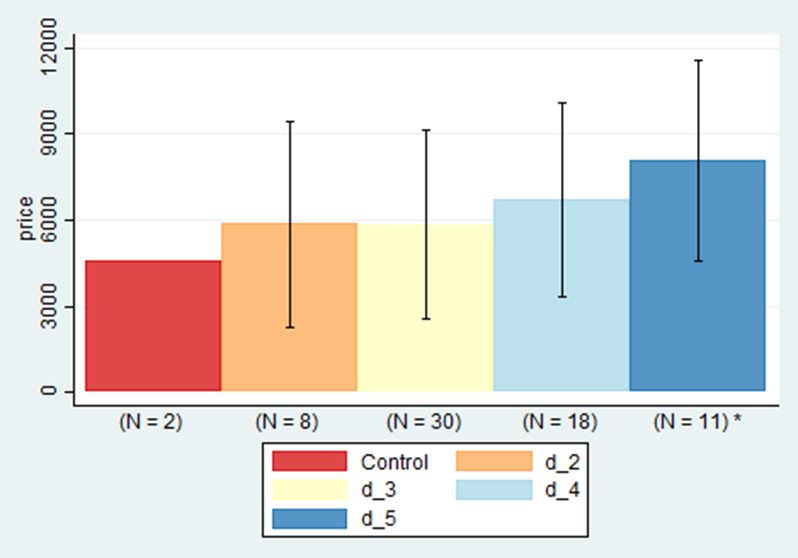
\includegraphics[width=\textwidth]{Raw/iegraph.png}
	+color(CornflowerBlue)(\caption{+textit(Add_a caption)})
	\end{figure}
	\end{Verbatim}
\end{center}

\section*{Exercise 5. Update {\LaTeX} file after making changes to the data}
Change your dataset by dropping all observation of Latin American countries. Rerun the codes for your tables and graphs with the same export path. Update {\LaTeX} file to view changes.

\begin{center}
	\textcolor{BurntOrange}{\emph{Tip:} before compiling the {\LaTeX} file with your updated tables and graphs, you should change the name of the PDF document with the old ones. Otherwise it will just save the new version over it when you compile.}
\end{center}

\section*{Exercise 6. (CHALLENGE) Using a do-file to edit a .tex file after exporting it}

This exercise requires more familiarity with {\LaTeX} than the previous. Don't worry if you can't complete it. \\

\textbf{Task 1:} Run the initial code for exercise 6 in the \textcolor{red}{Add path and name of do-file} do-file. This will create a table with sample sizes for control and treatment groups across regions and in the whole sample. Add this table to the .tex file you created in the previous exercises. How does that look?\\

\textbf{Task 2:} Open the \textcolor{red}{Add path and name of tex file} .tex file created by Stata. Can you identify the source of the extra spacing?\\

\textbf{Task 3:} Use the \texttt{filefilter} command in Stata to filter out the lines or characters in the fragmented file that create the extra spacing. Import the new .tex file and check how it looks.\\

\textbf{Task 4:} Repeat task 3 if necessary.

\end{document}          

